% !TEX encoding = UTF-8
% !TEX TS-program = pdflatex
% !TEX root = ../tesi.tex

%**************************************************************
\chapter{Analisi dei requisiti}
\label{cap:analisi}

Il primo giorno di stage il tutor aziendale ha indetto una riunione con tutti i dipendenti per definire le funzionalità del prodotto che dovevo sviluppare. Attraverso questo \emph{brainstorming} ho potuto farmi un'idea più precisa del compito a me assegnato, iniziando così la mia prima attività, cioè l'analisi dei requisiti. In accordo con il tutor non ho dovuto stilare un documento formale che comprendesse i casi d'uso, ma solo una lista di requisiti funzionali che il prodotto avrebbe dovuto soddisfare.

\section{Tracciamento dei requisiti}
Nella tabella che seguono verranno presentati i principali requisiti individuati durante l’analisi del problema.
Ogni requisito individuato avrà un codice identificativo univoco così formato: \\
\centerline{R\{Importanza\}\{Codice\}} \\ 
dove:
\begin{itemize}
	\item \textbf{importanza} può assumere uno dei seguenti valori:
	\begin{itemize}
		\item \textbf{O}: indica un requisito obbligatorio;
		\item \textbf{D}: indica un requisito desiderabile;
	\end{itemize}
	\item \textbf{codice} indica il codice identificativo del requisito, è univoco e deve essere
identificato in forma gerarchica.
\end{itemize}

\normalsize
\begin{longtable}{|c|>{\centering}m{7cm}|c|}
\hline
\textbf{Id Requisito} & \textbf{Descrizione} & \textbf{Importanza}\\
\hline
\endhead
RFO1 & Il sistema deve permettere all'utente di autenticarsi come amministratore o riconoscerlo come ospite dell'azienda. & Obbligatorio\\ 
\hline
\end{longtable}

\section{Analisi di mercato}
Il primo passo da compiere per iniziare lo sviluppo de prodotto è stato scegliere la piattaforma di \gls{NLP} migliore in base ai requisiti imposti dall'azienda. Le richieste fatte da \azienda{} riguardanti questo strumento erano le seguenti:
\begin{itemize}
	\item \textbf{costo}: il prezzo per il suo utilizzo doveva essere uguale a 0;
	\item \textbf{lingua}: deve supportare sia la lingua italiana, visto che al momento attuale i \gls{chatbot} sono implementati solo con quella;
	\item \textbf{documentazione}: il servizio deve essere ben documentato per permettere all'azienda, una volta finito il periodo di stage, di imparare ad utilizzarlo velocemente.
\end{itemize}

Questa attività di analisi di mercato si è rivelata quindi fondamentale per la buona riuscita del progetto, visto l'importanza che questo strumento avrebbe avuto nell'intero periodo di sviluppo. Le piattaforme da me studiate e analizzate sono riportate di seguito.

\subsubsection{IBM Watson Conversation}
IBM Watson Conversation\footcite{watson} è un prodotto della piattaforma IBM Watson, che attraverso IBM Cloud dà la possibilità di integrare i più potenti mezzi di AI nelle tue applicazioni. Il servizio di Conversation, oltre alla possibilità di creare \gls{chatbot} e agenti virtuali, può essere istruito ed interrogato per analizzare il testo posto in input, attraverso le \gls{API} messe a disposizione.\\
È possibile infatti creare dei workspace dedicati dove, attraverso \emph{intent} ed \emph{entities} creati e gestiti dallo sviluppatore, analizzare le domande poste dagli utenti, estraendo i dati che più interessano. L'integrazione con l'applicativo aziendale risultava semplice, grazie al SDK di Java\footcite{watsonSDK} messo a disposizione da IBM.

\begin{figure}[h]
	\centering
	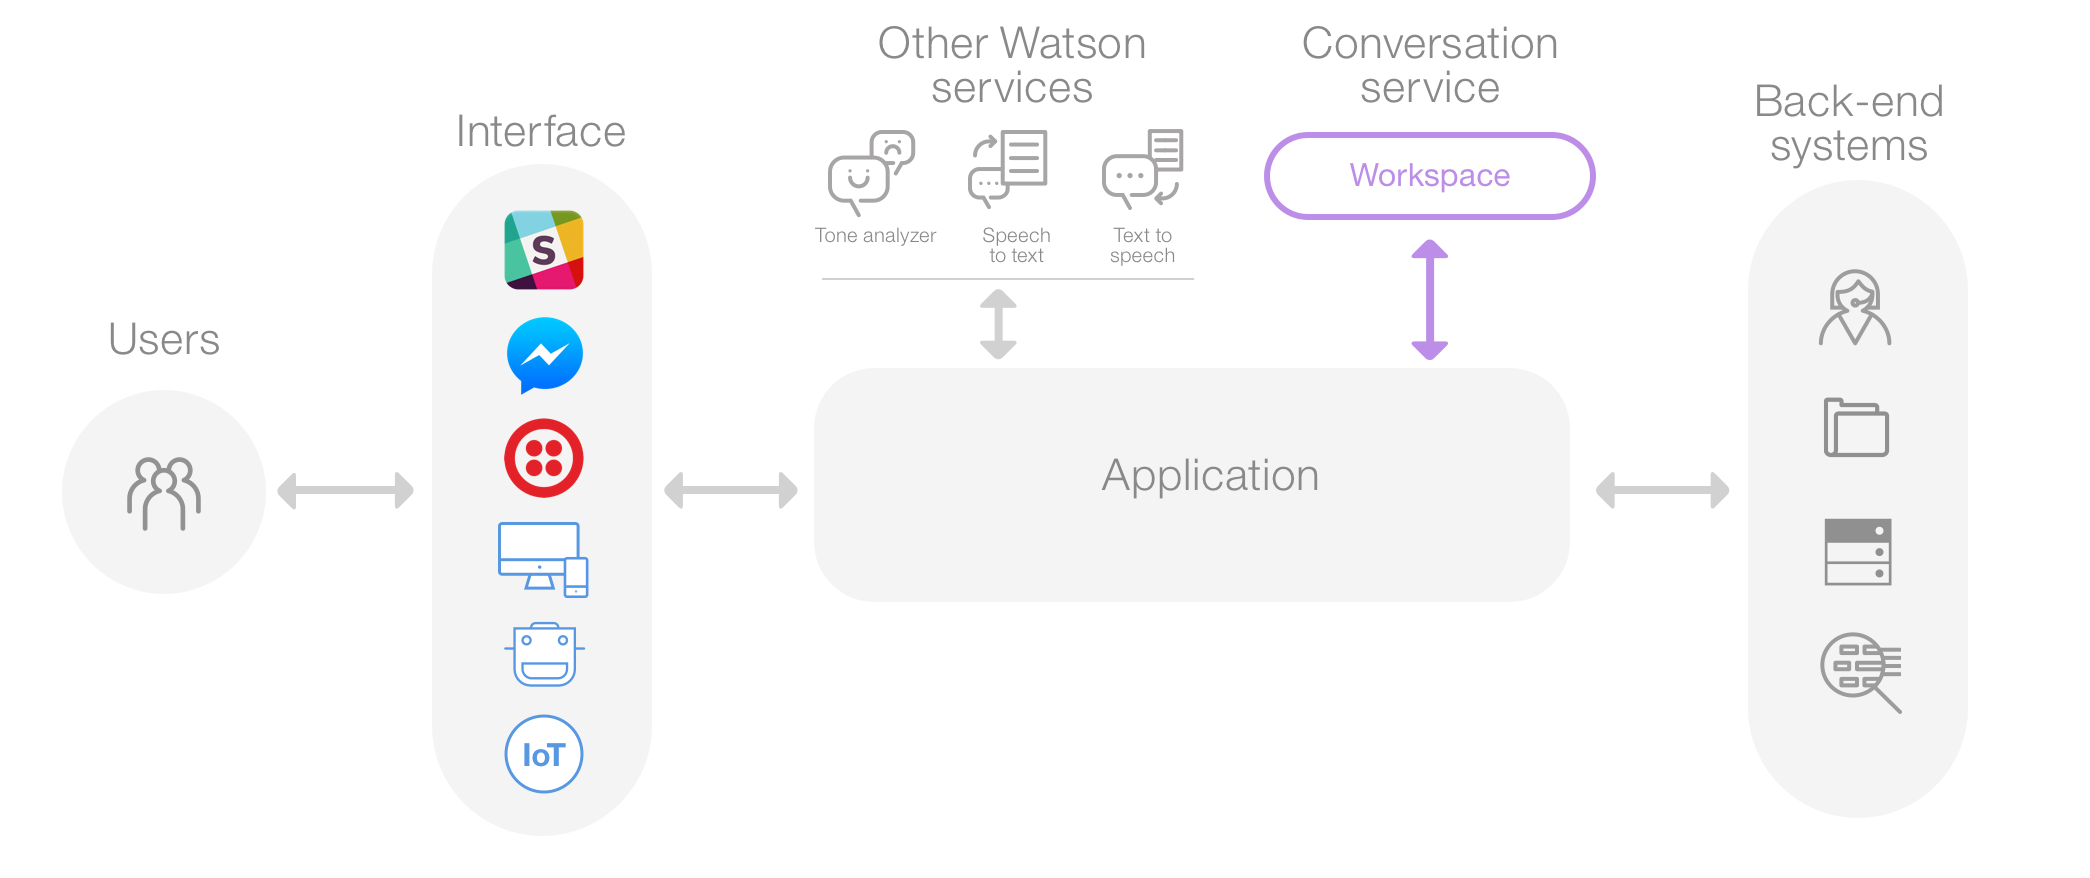
\includegraphics[scale=0.15]{../Immagini/conversation_arch_overview.png}
	\caption{Funzionamento IBM Watson Converation}
\end{figure}

Per quanto riguarda le richieste dell'azienda:
\begin{itemize}
	\item la \textbf{lingua italiana} è supportata, e non in versione beta;
	\item la \textbf{documentazione} è chiara ed esaustiva, con dei video di esempio molto utili;
	\item esiste un piano di \textbf{costi} gratis, chiamato \emph{Lite}, che però dà la possibilità di creare un numero limitato di \emph{workspace}, \emph{intent} ed \emph{entity}, risultando troppo vincolante per i futuri utilizzi aziendali. Le soluzioni a pagamento non sono state prese in considerazione in quanto non percorribili per l'azienda, almeno in un primo momento di utilizzo di questi servizi.
\end{itemize}

\begin{figure}[h]
	\centering
	
\includegraphics[scale=0.1]{../Immagini/watson_conversations_icon.png}
	\caption{Logo di IBM Watson Conversation}
\end{figure}

\subsubsection{wit.ai}
wit.ai\footcite{witai} è una società nata nell'ottobre del 2013 e acquisita da Facebook Inc. nel 2015.
L'obiettivo di wit.ai è quello di semplificare la creazione di applicazioni che prevedono interazioni testuali o vocali; per farlo viene messa a disposizione degli sviluppatori una piattaforma di linguaggio naturale aperta ed estensibile che ha la peculiarità di apprendere tramite ogni interazione eseguita.\\
wit.ai mette a disposizione un SDK gratuito ed \emph{open source} per il riconoscimento del linguaggio
naturale. Questa piattaforma è caratterizzata dall'utilizzo di \emph{context}, \emph{intent} ed \emph{entity} che sono
dei costrutti messi a disposizione per tradurre le richieste vocali dell'utente in dati processabili. In particolare il \emph{context} si utilizza per monitorare lo stato della conversazione tra l'utente e wit.ai.

\begin{figure}[h]
	\centering
	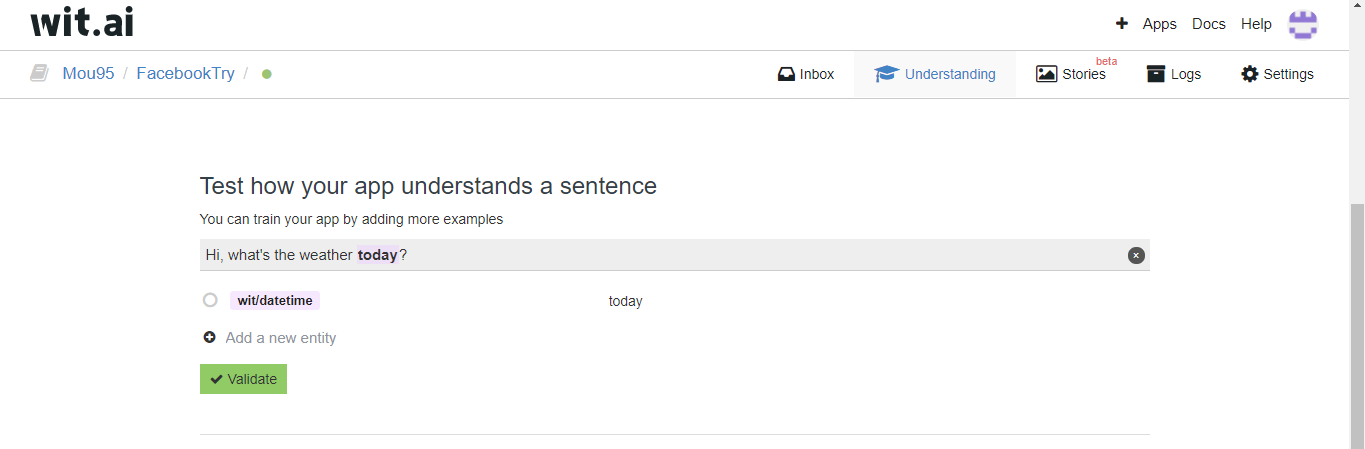
\includegraphics[scale=0.4]{../Immagini/witai_example.png}
	\caption{Esempio di creazione di un intento in wit.ai}
\end{figure}

Per quanto riguarda le richieste dell'azienda:
\begin{itemize}
	\item la \textbf{lingua italiana} è supportata;
	\item la \textbf{documentazione} è chiara ed esaustiva;
	\item l'utilizzo di wit.ai è completamente gratuito per progetti sia pubblici che privati.
\end{itemize}

Dal punto di vista tecnico l'unica mancanza di questo strumento, che ha influito nella decisione di non adottarlo, è la impossibilità di impostare delle \emph{required entity} all'interno degli \emph{intent}. Questo aspetto obbliga lo sviluppatore a introdurre dei controlli a livello di \emph{business logic}, che altrimenti non sarebbero necessari, come nel caso di altre piattaforme che saranno esposte successivamente.

\begin{figure}[h]
	\centering
	
\includegraphics[scale=0.5]{../Immagini/witai.png}
	\caption{Logo di wit.ai}
\end{figure}

\subsubsection{Microsoft LUIS}
Microsoft LUIS (Language Understanding Intelligent Service)\footcite{luis} è un prodotto di \emph{Microsoft Azure}, dedicato a comprendere le richieste di una persona tramite un \emph{language model} (entity/intent). \\
Come nelle altre piattaforme lo sviluppatore può creare degli \emph{intents}, cioè delle categorie di azioni che l'utente può intraprendere, dove nelle frasi ad esse correlate vengono evidenziate le \emph{entities}, ossia i pezzi di informazione di interesse, per poi gestirle nella logica del \gls{chatbot}. LUIS inoltre mette a disposizione la possibilità di "marcare" le \emph{entity} come \emph{required}, al contrario di wit.ai, e anche la creazione di cosiddette \emph{composite entities}, che possono essere intese come il raggruppamento di più \emph{entity} in una unica.
\begin{figure}[h]
	\centering
	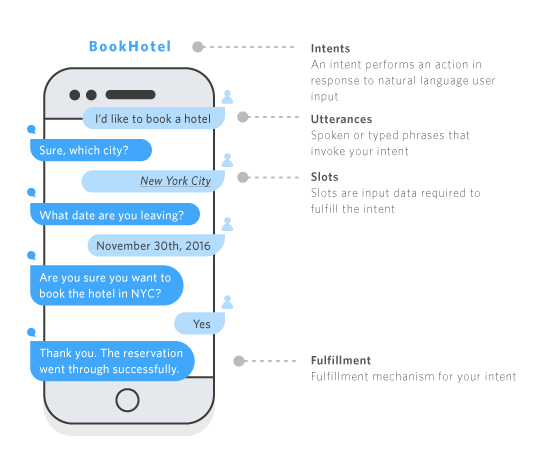
\includegraphics[scale=0.5]{../Immagini/lex_example.png}
	\caption{Utilizzo di Amazon Lex}
\end{figure}
Per quanto riguarda le richieste dell'azienda:
\begin{itemize}
	\item la \textbf{lingua italiana} è supportata;
	\item la \textbf{documentazione} è abbastanza chiara;
	\item esiste un piano \textbf{gratuito} di utilizzo di LUIS, con una limitazione del numero di chiamate alle API.
\end{itemize}

\begin{figure}[h]
	\centering
	
\includegraphics[scale=0.25]{../Immagini/luis.jpg}
	\caption{Logo di Microsoft LUIS}
\end{figure}

\subsubsection{Amazon Lex}
Amazon Lex\footcite{lex} è un servizio per la creazione di interfacce di comunicazione tramite voce e testo per qualsiasi tipo di applicazione. Amazon Lex offre funzionalità avanzate di apprendimento approfondito per il riconoscimento vocale e la dettatura, nonché per il riconoscimento del linguaggio naturale e la comprensione di testi, consentendo la creazione di applicazioni coinvolgenti e conversazioni realistiche. Con Amazon Lex, le stesse tecnologie di apprendimento approfondito su cui si basa \emph{Amazon Alexa} sono disponibili a tutti gli sviluppatori, consentendo così la creazione di \gls{chatbot} sofisticati e naturali in modo semplice e veloce.\\
L'interfaccia grafica consente ci creare i propri intents in modo intuitivo, seguendo le linee generali delle altre piattaforme.

Per quanto riguarda le richieste dell'azienda:
\begin{itemize}
	\item la \textbf{lingua italiana} è supportata;
	\item la \textbf{documentazione} non è chiara, sopratutto per quanto riguarda la creazione di \emph{intent}, \emph{entity} e \emph{utterance};
	\item esiste un piano \textbf{gratuito} per il primo anno di utilizzo di Amazon Lex. Finito questo tempo, la piattaforma diventa a pagamento, in proporzione al numero di chiamate effettuate.
\end{itemize}

\begin{figure}[h]
	\centering
	
\includegraphics[scale=0.5]{../Immagini/amazon-lex.png}
	\caption{Logo di Amazon Lex}
\end{figure}

\subsubsection{Api.ai}
Api.ai\footcite{apiai} è uno degli strumenti con il maggior numero di \emph{features} per quanto riguarda il \emph{machine learning} e il \gls{NLP}. Una volta acquistato da Google nel 2016 il suo volume di utilizzatori è aumentato in maniera esponenziale. \\
Api.ai fornisce SDK per i principali linguaggi di programmazione tra i quali \emph{C++, C\#, Java, Node.js, JavaScript} e \emph{Python}. Inoltre può essere integrato con \emph{Amazon Echo} e \emph{Microsoft Cortana}. Le applicazioni sviluppate su questa piattaforma sono costituite da \emph{agent}, i quali si occupano di trasformare il linguaggio naturale in dati processabili. Tali \emph{agent} sono a loro volta costituiti da \emph{intent}, che hanno il compito di associare la richiesta dell'utente ad una determinata azione del software, ed \emph{entity}, che sono strumenti per estrarre dal linguaggio naturale i parametri attesi.

Per quanto riguarda le richieste dell'azienda:
\begin{itemize}
	\item la \textbf{lingua italiana} è supportata;
	\item la \textbf{documentazione} è molto chiara;
	\item il suo utilizzo è gratuito, con delle limitazioni per il numero di richieste al minuto, ora, giorno e mese.
\end{itemize}

\begin{figure}[h]
	\centering
	
\includegraphics[scale=0.25]{../Immagini/apiai.png}
	\caption{Logo di api.ai}
\end{figure}

\subsection{Conclusioni dell'analisi}
Dopo una mia attenta analisi sui pregi e difetti di tutti gli strumenti, in accordo con il tutor aziendale, è stata fatta una breve riunione con gli altri dipendenti, dove ho illustrato in modo sintetico i dati raccolti. Amazon Lex e IBM Watson Conversation sono stati considerati non adeguati per lo sviluppo de progetto a causa dei loro costi, mentre le altre piattaforme, non presentando queste limitazioni, potevano essere tutte adottate. \\
La mia proposta è stata quella di utilizzare Api.ai, per la maggiore stabilità rispetto a wit.ai, per il maggior numero di lingue disponibili in vista di un supporto futuro ad interazioni con utenti di diversa nazionalità e per la maggiore maturità della piattaforma. L'azienda dopo aver valutato anch'essa i dati raccolti ha deciso di approvare la mia proposta, in quanto api.ai rispettava tutte le sue richieste iniziali, mostrando delle potenzialità molto interessanti per lo sviluppo del prodotto.